\RequirePackage{plautopatch}
\documentclass[dvipdfmx]{jsarticle}
%
\input preamble.tex

%
\title{モナド}
\author{ぱて(@pte\_hs)}
\date{\today}
\begin{document}
\maketitle
% 
%

\section{まえがき}
LaTeXの練習を兼ねて,最近学んでいるモナドについて整理しようと考えた.

\section{準備運動}
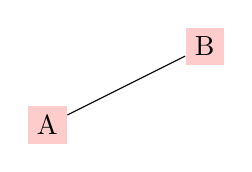
\begin{tikzpicture}
  \node[fill=red!20] (hoge) at (0,0) {A};
  \node[fill=red!20] (fuga) at (2,1) {B};
  \draw (hoge) --(fuga);
\end{tikzpicture}




%
%
\end{document}